\documentclass[11pt]{standalone}
\usepackage{amssymb}
\usepackage{amsmath}
\usepackage[no-math]{fontspec}
\usepackage{unicode-math}
\usepackage{libertinus}
\usepackage{pgf,xcolor}
\usepackage{tikz}
\usetikzlibrary{arrows.meta, backgrounds}
\usepackage{pgfplots}
\pgfplotsset{compat=newest}

\setmainfont{Libertinus Serif}
\setmathfont{Libertinus Math}

\definecolor{my_darkgray}{HTML}{484949}
\definecolor{my_lightgray}{HTML}{F3F4F4}
\definecolor{my_darkblue}{HTML}{005A94}
\definecolor{my_lightblue}{HTML}{CCDEE9}
\definecolor{my_yellow}{HTML}{FFEC7F}
\definecolor{my_red}{HTML}{E60000}
\definecolor{my_orange}{HTML}{E87846}

\begin{document}

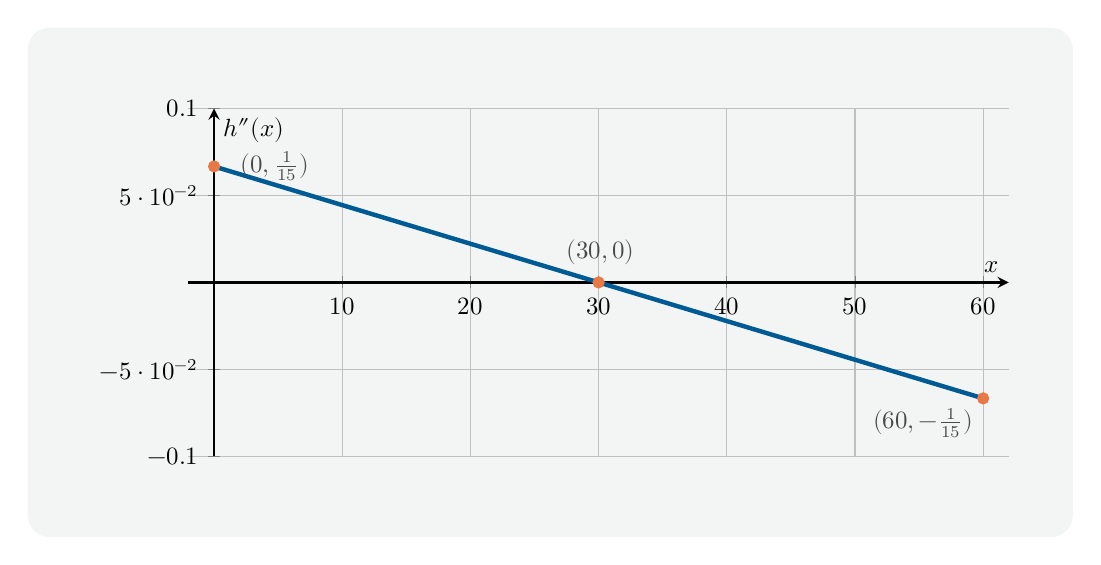
\begin{tikzpicture}[
    show background rectangle,
    background rectangle/.style={fill=my_lightgray, rounded corners=8pt},
    inner frame sep=0.8cm
]

\begin{axis}[
    width=12cm,
    height=6cm,
    axis lines = center,
    xlabel = {$x$},
    ylabel = {$h''(x)$},
    xmin=-2, xmax=62,
    ymin=-0.1, ymax=0.1,
    grid = both,
    % Omit axis equal here so that the line and points are clearly visible
    axis line style={thick},
    ticklabel style={font=\small},
    label style={font=\small},
]

% second derivative h''(x) = 1/15 - x/450 on [0, 60]
\addplot[
    draw=my_darkblue,
    ultra thick,
    samples=300,
    domain=0:60
]
{0.0666666667 - 0.00222222222*x};

% mark value at x = 0: h''(0) = 1/15 ≈ 0.0667
\addplot[
    only marks,
    mark=*,
    mark size=2pt,
    draw=my_orange,
    fill=my_orange
]
coordinates {(0,0.0666666667)};

\node[anchor=west, font=\small, my_darkgray]
at (axis cs:1,0.0666666667) {$\,(0, \tfrac{1}{15})$};

% mark value at x = 30: h''(30) = 0
\addplot[
    only marks,
    mark=*,
    mark size=2pt,
    draw=my_orange,
    fill=my_orange
]
coordinates {(30,0)};

\node[anchor=north, font=\small, my_darkgray]
at (axis cs:30,0.03) {$\,(30, 0)$};

% mark value at x = 60: h''(60) = -1/15 ≈ -0.0667
\addplot[
    only marks,
    mark=*,
    mark size=2pt,
    draw=my_orange,
    fill=my_orange
]
coordinates {(60,-0.0666666667)};

\node[anchor=north east, font=\small, my_darkgray]
at (axis cs:60,-0.0666666667) {$(60, -\tfrac{1}{15})$};

\node[anchor=south, font=\small\bfseries, my_darkgray]
at (rel axis cs:0.5,0.98)
{Second derivative $h''(x) = \dfrac{1}{15} - \dfrac{x}{450}$};

\end{axis}

\end{tikzpicture}

\end{document}